\documentclass[conference,a4paper,flushend]{cs-techrep}
\pdfoutput=1 % pdflatex hint for arxiv.org (within first 5 lines)

% Class cs-techrep.cls loads biblatex / biber with predefined options
\addbibresource{embedded.bib}       % its content is declared below, embedded within this tex-file
\addbibresource{webdev_commons.bib} % includes REST, React, Angular, Vue, Svelte, Docker, AWS-*, Socket.IO, and many more!
\addbibresource{cpn_all_all.bib}    % includes all previous CyberLytics@OTH-AW technical reports

% ======================================================================
% EDIT THESE:

\cstechrepAuthorListTex{Sebastian Weidner, Jonas Hermann, Nils Bayerl, Dominik Schwagerl, \\ Timon Spichtinger, Christoph P.\ Neumann\,\orcidlink{0000-0002-5936-631X}}
\cstechrepAuthorListBib{Sebastian Weidner and Jonas Hermann and Nils Bayerl and Dominik Schwagerl and Timon Spichtinger and Christoph P. Neumann}

% Capitalization: https://capitalizemytitle.com/style/Chicago/
\cstechrepTitleTex{InfluenzaConnect: Eine React-basierte Webanwendung für Influencer-Marketing}
 % IF you need manual linebreaks in the titel, then clone the title without linebreaks for BibTeX:
\cstechrepTitleBib{{\cstechrepTitleTex}}

\cstechrepDepartment{CyberLytics\-/Lab at the Department of Electrical Engineering, Media, and Computer Science}
%\cstechrepDepartment{CyberLytics\-/Lab an der Fakultät Elektrotechnik, Medien und Informatik} % DE
\cstechrepInstitution{Ostbayerische Technische Hochschule Amberg\-/Weiden}
\cstechrepAddress{Amberg, Germany}
%\cstechrepAddress{Amberg, Deutschland} % DE
\cstechrepSeries{Technical Reports}
%\cstechrepSeries{Technische Berichte} % DE
\cstechrepYear{2024}
\cstechrepMonth{3}
\cstechrepNumber{CL-\cstechrepYear{}-42}
%\cstechrepLang{english}  % en-US
\cstechrepLang{ngerman} % DE

% Special remark on babel/csquotes terminology in regard with US-vs-UK:
% en-US  = [english]/[american]/[usenglish] (+ [canadian])
% en-UK  =           [british] /[ukenglish] (+ [australian]) <OXFORD>
% For cs-techrep (like ACM), the recommended english variant is en-US!

% DO NOT DELETE THIS:
\filecontentsForceExpansion|[] % force command expansion inside a filecontents* environment
\begin{filecontents*}[overwrite]{selfref.bib}
    @TECHREPORT{selfref,
        author = {|cstechrepAuthorListBib},
        title  = {\cstechrepTitleBib},
        institution = {\cstechrepInstitution, \cstechrepDepartment},
        series = {\cstechrepSeries},
        number = {\cstechrepNumber},
        year   = {|cstechrepYear},
        month  = {|cstechrepMonth},
        langid  = {|cstechrepLang},
    }
\end{filecontents*}

% ======================================================================
% EDIT THIS:

\begin{filecontents}[overwrite]{embedded.bib}
@online{ieee2015howto,
    author = {Michael Shell},
    title = {How to Use the {IEEEtran} \LaTeX\ Class},
    url = {http://mirrors.ctan.org/macros/latex/contrib/IEEEtran/IEEEtran_HOWTO.pdf},
    year = {2015}
}
@online{ieee2018formattingrules,
    author = {{IEEE}},
    title = {Conference Template and Formatting Specifications},
    url = {https://www.ieee.org/content/dam/ieee-org/ieee/web/org/conferences/Conference-template-A4.doc},
    year = {2018}
}
@online{iaria2014formattingrules,
    author = {{IARIA}},
    title = {Formatting Rules},
    url = {http://www.iaria.org/formatting.doc},
    year = {2014}
}
@online{iaria2009editorialrules,
    _author = {Cosmin Dini},
    author = {{IARIA}},
    title = {Editorial Rules},
    url = {https://www.iaria.org/editorialrules.html},
    year = {2009}
}
@online{languagetool,
    author = {{LanguageTooler GmbH}},
    title  = {{LangueTool}},
    url    = {https://languagetool.org/overleaf}
}
@online{overleaf,
    author = {{Digital Science UK Limited}},
    title  = {{Overleaf}},
    url    = {https://www.overleaf.com}
}
\end{filecontents}

\usepackage{fontawesome} % i.a., \faWarning{}
\usepackage{relsize}     % i.a., \textsmaller{...}
\usepackage{lipsum}      % for blindtext

% ======================================================================

% cf. https://ctan.org/pkg/acronym
% Usage:
% singular, within sentence       = \ac{gui}
% singular, beginning of sentence = \Ac{gui}
% plural, within sentence         = \acp{gui}
% plural, beginning of sentence   = \Acp{gui}
\begin{acronym}
    \acro{gui}[GUI]{Graphical User Interface}
    \acro{ide}[IDE]{Integrated Development Environment}
\end{acronym}

% https://www.silbentrennung24.de/
% https://www.hyphenation24.com/
\hyphenation{block-chain block-chains Ethe-re-um}
\begin{document}
\selectlanguage{\cstechrepLang}

\maketitle

\begin{abstract}
% Referenz React, MongoDB, Docker, Flusk, Tailwind CSS; axios, fetch
\textit{InfluenzaConnect ist eine Webandwendung, die das Ziel der strategische Vernetzung von Unternehmen und Influencern verfolgt. Dabei soll das Influencer Marketing von Unternehmen, als auch die selbstständige Vermarktung als Influencer erleichtert werden. Die Besonderheit von InfluenzaConnect ist u.a. die automatisierte Analyse des Instagram-Profils des Influencers bei der Registrierung.\\
% Durch InfluenzaConnect soll das Influencer-Marketing für Unternehmen effizienter gestaltet werden. Gleichzeitig bietet die Plattform den Influencern eine bequeme Möglichkeit, sich im Web zu präsentieren.
%Um eine große Reichweite zu erzielen, wurde InluenzaConnect als Webandwenung realisiert. 
Die Architektur basiert im Frontend auf dem React JavaScript-Framework, im Backend auf dem Python-Framework Flusk und für die Persistenz wird die NoSQL Datenbank MongoDB verwendet. 
Frontend, Backend und die MongoDB wurden mittels Docker containerisiert, um eine hochskalierung der Webanwendung zu ermöglichen.
Als CSS Framework wurde Tailwind CSS und für die Kommunikation zwischen Frontend und Backend die Axios, ein Promise-basierter HTTP-Client sowie die Fetch API verwendet. Für die Datenaquise wurde auf die Instagram-API und ? zurückgegriffen.}
\end{abstract}
% A list of IEEE Computer Society appoved keywords can be obtained at
% http://www.computer.org/mc/keywords/keywords.htm
\begin{IEEEkeywords}
Influencer-Marketing; WebApp; Business; SocialMedia.
\end{IEEEkeywords}




%#################### Einleitung ###########################
\section{Überblick}
%------------------- Motivation ----------------------------
\subsection{Motivation}
Unternehmen wollen möglichst viele ihrer Produkte verkaufen. Dazu braucht es eine gute Qualität der Produkte, preiswerte Verkaufspreise und Markenbekanntheit. Letzteres erfordert ein ausgereiftes Marketing-Konzept.
Ein Marketing-Konzept ist dabei das Influencer-Marketing. Beim Influencer-Marketing lassen Unternehmen ihre Produkte von Influencern bewerben, um den Bekanntheitsgrad der Firma, sowie den Bekanntheitsgrad und die Umsatzzahlen ihrer Produkte weiter zu erhöhen. 

Was ist das Problem?\\
Unternehmen wollen authentische, sowie glaubwürdige Stimmen von Menschen finden, die ihr Produkt präsentieren und bewerben können. Die Lösung auf dieses Problem ist das Influencer-Marketing. Dieses ist aber noch nicht so weit verbreitet und Unternehmen, die sich für dieses Marketing-Konzept entschieden haben, stehen wieder vor neuen Problemen.

\begin{enumerate}

\item{Wie finde ich den passenden Influencer für meine Produkte?}
\item{Es ist aufwending mit mehreren Influencern zu verhandeln --> Wie kann ich mit mehreren Influencern effizient verhandeln?}
\item{Welche Social-Media-Plattformen kommen für das Bewerben meiner Produktes infrage, bzw. wie finde ich die richtige Plattform für meine Produkte? Soll es Instagram, Facebook, TikTok, YouTube, Pinterest, X, LinkedIn oder doch ein privater Blog sein, um nur einen Einblick über die Vielfalt der Plattformen zu bieten. \\}

Dazu kommen generelle Probleme wie:

\item{Es gibt noch nicht viele Influencer die im B2B-Space tätig sind.}
\item{Es gibt viele unbekannte Influencer.}
\item{Influencer mit hohen Reichweiten sehen sich selbst gar nicht als Influencer an.}
\item{Influencer mit kleineren Reichweiten sind schwer auffindbar und haben es schwerer, Aufträge von Unternehmen zu bekommen.}

\end{enumerate}

Durch unsere Webbasierte Influencer-Marketing-Plattform wollen wir es schaffen, diese Probleme zu beheben und das Influencer-Marketing zu vereinfachen.

%------------------- MVP --------------------------------
\subsection{MVP}
Das MVP umfasst folgende Anforderungen:
\begin{enumerate}
\item{\textit{Registrierungs- und Anmeldungsseite für Influencer}}
\item{\textit{Automatische Analyse des Instagram-Profils des Influencers}}
\item{\textit{Tabellarische Übersicht aller registrierten Influencer, inkl. Sortierung, Suche und Filterungsfunktion}}
\item{\textit{Datailübersicht zum Influencer mit allen relevanten Informationen}}
\end{enumerate}

%------------------- Implementierungsstand --------------------------------
\subsection{Implementierungsstand}
Vom MVP wurden folgende Punkte umgesetzt:
\begin{enumerate}
\item{\textit{Registrierungs- und Anmeldungsseite für Influencer}}
\item{\textit{Automatische Analyse des Instagram-Profils des Influencers während der Registrierung}}
\item{\textit{Übersicht über alle registrierten Influencer, inkl. Suche und Spaltenfilter}}
\end{enumerate}

Die \textit{Datailübersicht zum Influencer} wurde nicht implementiert. Stattdessen wurde für den \textit{angemeldeten Influencer eine Profilseite implementiert, in der er seine aktuellen Profildaten einsehen und ändern kann}. Um alle Daten zum Influencer totz der fehlenden Dateilansicht für die Besucher der Website bereitzustellen, wurden diese vorerst in die Tabelle in der Übersichtsseite zu den Influencern integriert. \\


%#################### Architektur ###########################
\section{Architektur}

%------------------- Containerisierung --------------------------------
\subsection{Containerisierung}

%Bild vom Deployment
\begin{figure}[h]
	\centering
	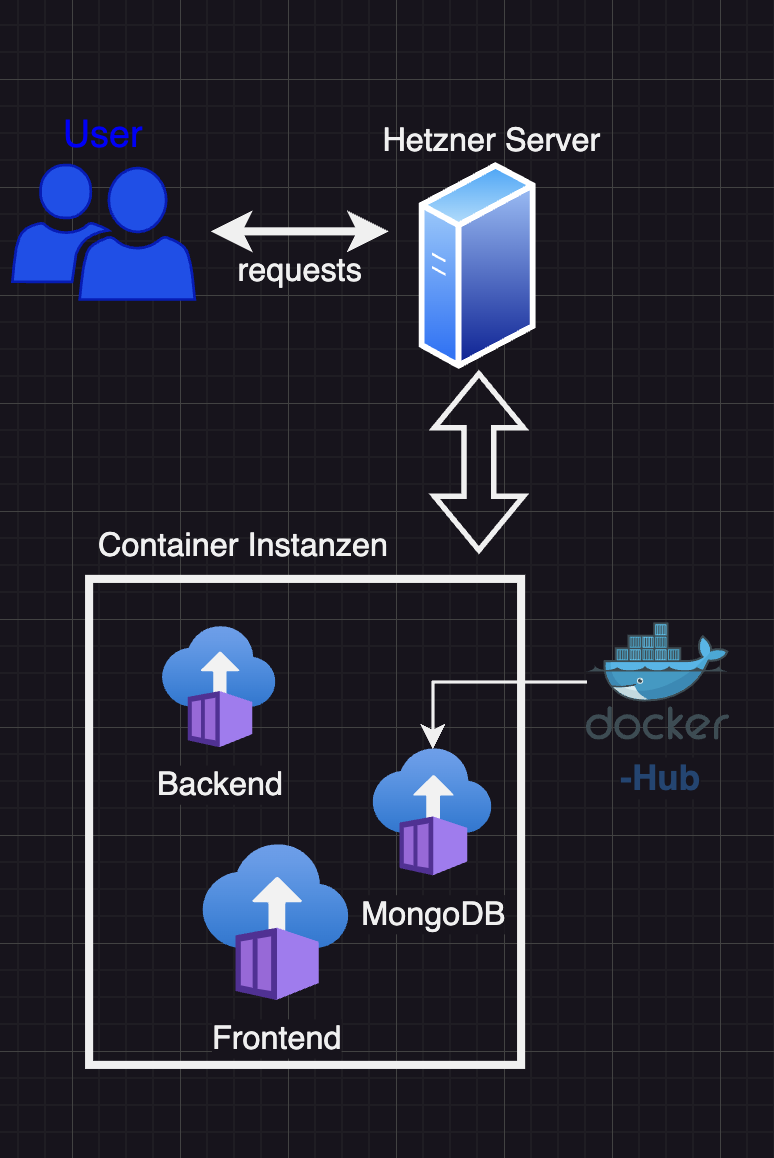
\includegraphics[width=\linewidth]{../Bilder/Deployment.png}
	\caption{Containerisierung und Deployment}
	\label{fig:Deployment}
\end{figure}

%Referenz Docker
Das Projekt wurde mittels Docker containerisiert, um eine flexible und skalierbare Umgebung für die verschiedenen Komponenten der Anwendung zu schaffen.
Dabei wurden das Frontend, Backend sowie die MongoDB in separate Docker-Container aufgeteilt, was eine einfache Verwaltung und Skalierung der einzelnen Dienste ermöglicht. Dockerfiles legen dabei fest, welche Software und Abhängigkeiten in den virtuellen Containern installiert werden. Für das Backend wird ein Python 3.10 Slim Image verwendet. In dieses werden beim Starten des Containers die notwendigen Python-Pakete automatisiert installiert und der Anwendungscode kopiert. Das Frontend basiert auf einem Node.js 16 Image, das ebenfalls automatisch die benötigten Node-Module installiert und den Build-Prozess des Frontends startet (Kein multi stage).

%------------------- Deployment --------------------------------
%Referenz Hetzner, Github, Git, GitHub Actions
\subsection{Deployment}
InfluenzaConnect verwendet GitHub als Git-Respository. Das Deployment in unsere Hetzner-Cloud erfolgt demnach mittels GitHub Actions. Der CD-Workflow befindet sich wird dabei ausgelöst, sobald Änderungen auf den \texttt{prod} Branch gepusht werden. Der anschließende Deployment-Job läuft auf einer Ubuntu-Maschine in der Hetzner-Cloud und umfasst folgende Schritte:
\begin{enumerate}
\item{\textbf{Checkout Code} - Der Quellcode wird aus dem Repository ausgecheckt.}
\item{\textbf{Setup SSH} - SSH wird eingerichtet, um eine sichere Verbindung zum Hetzner-Server
herzustellen.}
\item{\textbf{Deploy to Hetzner} - Der Code wird auf den Hetzner-Server deployt.}
\end{enumerate}
Beim deployen wird dabei unser Projektverzeichnis aktualisiert, Docker Compose verwendet, um die bestehenden Container zu stoppen, neu zu bauen und schließlich die Anwendung in die Produktionsumgebung hochzufahren.
Durch diese Pipline wird sichergestellt, dass jede Änderung im \texttt{prod} Branch automatisch auf dem Produktionsserver deployet wird. Dadurch wird eine kontinuierliche Integration und Bereitstellung neuer Features und Bugfixes ermöglicht, Entwicklungszyklen beschleunigt und die Qualität der Anwendung verbessert.


%#################### Techstack ###########################
\section{Techstack}

%Bild von Architektur
\begin{figure}[h]
	\centering
	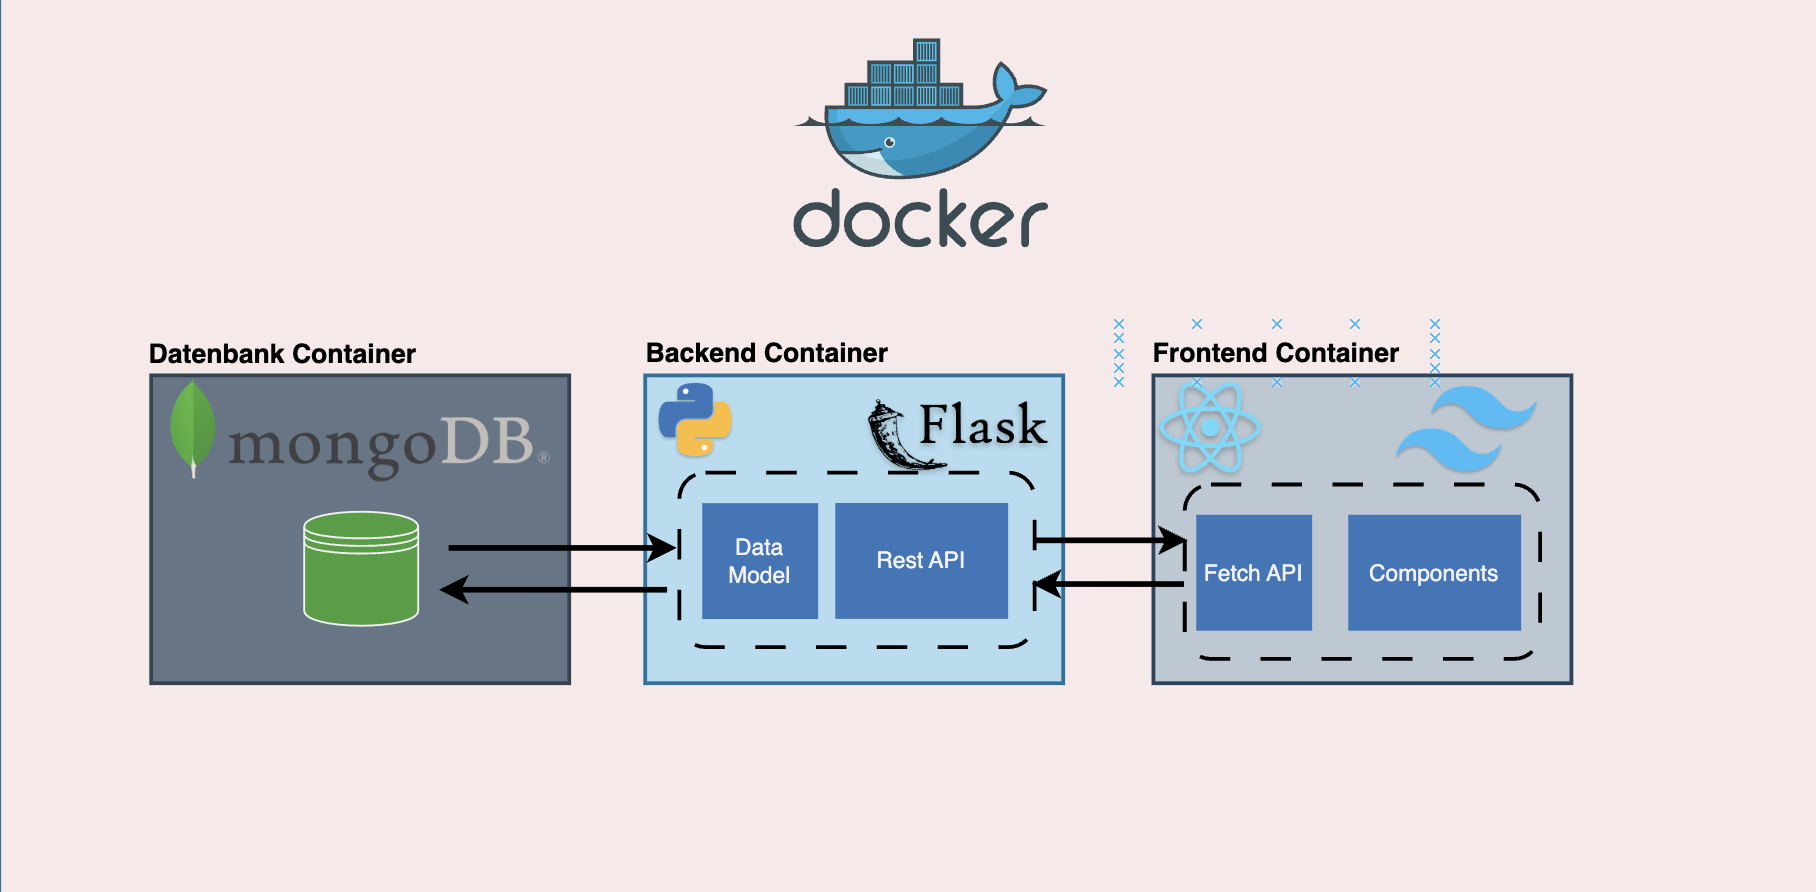
\includegraphics[width=\linewidth]{../Bilder/Architektur.png}
	\caption{Architektur von InfluenzaConnect}
	\label{fig:Architektur}
\end{figure}

\subsection{Frontend}
% Referenz React, Tailwind CSS, Typescript, 
Für die Realisierung des Frontends wird das JavaScript-Framework React verwendet. Es erleichtert die Entwicklungsarbeit im Frontend, indem es dabei hilft, wiederverwendbaren Code zu schreiben, sowie graphische Inhalte dynamisch aufzubauen und zu befüllen. HTML, CSS und JavaScript-Code wird dabei in sogenannten Komponenten gekapselt. In React gibt es sog. Hooks, die dazu benutzt werden, bestimmte Funktionialitäten in den Komponenten zu erreichen. Erwähnenswert ist hier der Hook \texttt{useState()}, der bestimmte Zustände zwschenspeichern kann, sodass diese beim erneuten Rendern der Komponente nicht verloren gehen. Desweiteren haben wir uns für die Gestaltung der Webpages für Tailwind CSS entschieden. Tailwind CSS wird oft mit React verwendet und ist zur Zeit sehr im Trend, weil es leicht zu erlernen ist, gutes vordefiniertes Design und trotzdem große Gestaltungsfreiräume bietet, da man notfalls interne CSS-Werte speziell für sein Projekt überschreiben kann. Außerdem haben wir entschlossen, anstatt JavaScript auf TypeScript zu setzen, da TypeScript eine Typisierung zulässt und somit logische Typfehler beseitigt. 

TypeScript ist komplett kompatibel mit JavaScript.
Fetch!!


\subsection{Backend}
%Referenz Python, Flusk, MongoDB, pymongo
Im Backend haben wir uns für das Python-Webframework Flask entschieden. Flask ermöglicht die Erstellung von Webanwendungen in Python durch eine minimalistiche und flexible Struktur, sodass es sich gut für kleine bis mittelgroße Projekte eignet. Durch das Definieren von Routen, basierend auf den Anforderungen der Clients werden die HTTP-Anfragen verarbeitet und entsprechende Antworten zurückgeben. 

\subsection{Persistenz}
Zum persistieren der Daten setzen wir auf eine MongoDB als Datenbanksystem. Die \texttt{pymongo}-Bibliothek von Python fungiert dabei als offizieller Treiber für die MongoDB, die Funktionen für die Interaktion der Datenbank bereitstellt, um Daten zu speichern, abzurufen, aktualisieren und zu löschen.




%#################### Implementierung ###########################
\section{Implementierung}
\subsection{Frontend}
%\begin{enumerate}
%\item{test}
%\end{enumerate}

\subsubsection{Landing Page\\}
 Routing auch mit erwähnen

\subsubsection{Registrierung\\}
Die Registrierung dient dazu, sich als Influencer registrieren und vermarkten zu können. Die Registrierung ist in drei Schritten aufgebaut:
Zuerst muss er seine Anmeldeinformationen - eingeben. Im Zweiten Schritt werden seine Persönliche Daten abgefragt, die später teilweise für die Unternehmen veröffentlicht werden und im Dritten Schritt muss er seinen Instagram-Account hinterlegen, der anschließend im Backend analysiert wird.\\
Nachfolgend finden Sie eine Detailierte Auslistung der Eingaben:
\begin{itemize}
\item{Anmeldeinformationen - Email, Passwort}
\item{Persönliche Daten - Anrede, Vorname, Nachname, Nationalität, Telefonnr., Gesprochene Sprachen, Beschreibung über sich selbst}
\item{Verknüpfung Socail-Media Accounts - Instagram Username}
\end{itemize}
Jeder der drei Schritte wurde in einem Eigenständigen Fomular realisiert, zwsichen denen durch einen Weiter- und Zurück-Button hin- und hergewechselt werden kann.

% Referenz React hook Form
Für die Eingabefelder wurden von Grund auf eigene Komponenten erstellt. Ein Eingabefeld besitzt immer ein Label und ein Ausgabefeld für Fehlermeldungen. Dabei taucht unter jedem Eingabefeld eine Fehlermeldung auf, falls die eingegebenen Daten nicht den Richtlinien entsprechen. 
Um das Datenhandling mit den Input-Felder zu vereinfachen und um Codezeilen zu sparren, wurde die Bibliothek \texttt{React Hook Form} im Frontend eingebunden. Durch diese kann man vereinfacht die Logik hinter den Formularen erstellen. %Die Formularfelder werden dabei an ein zentrales Formular-Objekt vom Typ \texttt{useForm()} gebunden, indem diese mit der Methode \texttt{register(\dq InputFeldName \dq )} daran gebunden werden.  \texttt{register(...)} setzt setzt die Methoden \texttt{onBlur() }, \texttt{onChange()}, sowie die Attribute \texttt{ref} und \texttt{name} des Eingabefelds. So können Formulareingaben 
Formulareingaben können so z.B. ganz einfach zwischenspeichert werden, um diese z.B. beim zurückgehen nicht zu verlieren. Auch das einbinden einer Datenvalidierung wird unterstützt. So werden die Eingaben mit der Bibliothek \texttt{Yup} validiert, die gleichzeitig das Setzten eigener Fehlermeldungen, nach jedem Validierungsschritt erlaubt. Die Fehlermeldungen werden anschließend in ein internes Objekt, dass \texttt{React Hook Form} zu jedem registrierten Input-Element erstellt, geschrieben und durch unsere Komponte automatisch unter dem Input-Feldern angezeigt. 

Wurden alle Eingaben getätigt werden diese gesammelt mittels \texttt{fetch()} API an das Backend gesendet und dort nochmals überpfrüft.
Neben einer einfachen Eingabefeld, wurden Komponenten für ein Select-, ein Multiselectdropdown und für zwei Buttons zur Registrierung erstellt. 



\subsubsection{An- und Abmeldung\\}
\texttt{
- Wiederverwendung der Input-Komponenten
- Popup-Dialog Komponente von XXX verwendet
- Daten ans Backend gesendet - Response - Session gesetzt 
- Button Logout und Email erscheint 
- Logout -> Session gelöscht, Erscheinungsbild wie zuvor
}
\subsubsection{Profildaten Bearbeiten\\}
\texttt{
- Anpassung der Input-Komponenten, Standardmäßig non-Editable
- Daten werden anhand der Email, die in der Session gespeichert ist rausgeholt.
- durch Edit-Button kann kann man die Eingabefelder bearbeiten. Gleichzeitig erscheint unten links ein Abbrechen- und ein Speichern-Button. Wird der letztere Button betätigt, werden die Daten im Frontend Validiert und anschließend ins Backend gesendet. Dort werden Sie nochmals auf validiert und schlussendlich persistiert, indem die alten mit den neuen Daten überschrieben werden.
}

\subsubsection{Influncerübersicht\\}
% Asynchroner Fetch? Datenfilterung überarbeiten 
Die Influencerübersicht dient dazu, dass Unternehmen einen passenden Influencer für sich finden können. Demnach sind in einer Tabelle alle Registrierten Influencer mit allen relevanten Daten, inkl. Informationen, die durch die Analyse des Instagram-Acounts gewonnen wurden zu sehen. %???
Für die Datendarstellung in der Tabelle wurde in TypeScript eine Datenstruktur erstellt, auf die die Daten vom Backend gamappt werden. %Die Daten werden im React-Hook \texttt{useEffect()}, der dazu dient die Komponente mit externen Systemen zu synchronisiern, vom Backend mittels \texttt{fetch()} API geholt.
\\
Ein \textbf{Spaltenfilter} ermöglicht es, Spalten ein- und wieder auszublenden. Die Komponente ist dabei so ähnlich wie das Multiselect-Dropdown in der Registrierung aufgebaut, nur das die Werte mittels einer Checkbox ausgewählt werden können und ausgewählte Einträge nicht außerhalb des Dropdowns sichtbar werden. Die Komponente wurde ohne \texttt{React Hook Form} realisiert. Stattdessen wird ihr eine \texttt{onChange()} Event-Handler übergeben, der die ausgewählten Spalten in einer Zustands-Variable vom Typ \texttt{useState<string[]>()} speichert. Vor dem Rendering der Spalten muss somit nur noch überprüft werden, ob die angegebene Spalte in dieser Varialbe enthalten ist. 
\\
Durch \textbf{Suchfeld} kann der User die Tabelle direkt nach dem Namen eines bestimmten Influencer durchsuchen. Dazu wird ebenfalls der Wert des Suchfeldes in eine Variable vom Typ \texttt{useState<string>()} gespeichert. Anschließend wird eine Filterfunktion mithilfe des Inhalts dieser Variable auf allen Daten angewendet und die Tabelle aktualisiert.


\subsection{Backend}
texttt{
Unser Backend ist mit Python und dem Framework FastAPI realisiert und fungiert als zentrale Schnittstelle zwischen Datenbank und Frontend. Über eine RESTful-API kommuniziert das Frontend mit dem Backend, wobei JSON als Rückgabeformat für alle API-Endpunkte verwendet wird.
}
Die Hauptaufgaben des Backends umfassen die Aufbereitung und Bereitstellung von Daten für das Frontend sowie die Verarbeitung von Benutzeranfragen. Dabei haben wir uns für das Python-Webframework Flask entschieden. Flask ermöglicht die Erstellung von Webanwendungen in Python durch eine minimalistiche und flexible Struktur, sodass es sich gut für kleine bis mittelgroße Projekte eignet. Durch das Definieren von Routen, basierend auf den Anforderungen der Clients werden die HTTP-Anfragen verarbeitet und entsprechende Antworten zurückgeben. In unserem Fall haben wir folgende Routen definiert:

\begin{table}[h]
    \centering
    \begin{tabular}{|l|>{\raggedright\arraybackslash}m{0.75\linewidth}|}
        \hline
  	 \multicolumn{1}{|c|}{\textbf{Route}} & \multicolumn{1}{c|}{\textbf{Zweck der Route}} \\
        \hline
        \verb|/signup| & Registrierung: Die eingegebenen Daten werden validiert und verschlüsselt in der MongoDB gespeichert. \\
        \hline
        \verb|/login| & Anmeldung: Die Eingaben werden überprüft, und bei erfolgreicher Authentifizierung eine Session gestartet. \\
        \hline
        \verb|/profile| & Profildaten ändern: Gibt die Profilinformationen des eingeloggten Benutzers zurück. \\
        \hline
        \verb|/logout| & Abmelden: Beendet die aktuelle Sitzung und meldet den Benutzer ab. \\
        \hline
        \verb|/collect| & Influencer Übersichtstabelle: Gibt die Daten aller registrierten Influencer gesammelt zurück, um diese im Frontend anzuzeigen \\
        \hline
	   \verb|/<session>| & Routen für Session-Handling \\
        \hline
    \end{tabular}
    \caption{Definierte API-Routen}
    \label{tab:api-routes}
\end{table}



\subsubsection{Datenvalidierung und -speicherung}
Die Validierungsfunktionen prüfen die Benutzereingaben mithilfe von regulären Ausdrücken und einfachen Bedingungen, um sicherzustellen, dass sie den erwarteten Standards entsprechen. Dabei wird z.B. überprüft, ob die E-Mail im richtigen Format vorliegt, das Passwort ausreichend lang ist oder obligatorische Informationen wie Vor- und Nachname korrekt angegeben wurden. Spezielle Validierungen wie die Überprüfung des Instagram-Benutzernamens und optionaler Informationen wie der Telefonnummern werden ebenfalls durchgeführt. Darüber hinaus nutzen diese Funktionen externe Ressourcen, beispielsweise eine Webanfragen für die Überprüfung von Instagram-Benutzernamen auf ihre Existenz und ob es sich um ein privates oder öffentliches Profil handelt. 




\subsubsection{Session}
In unserer Flask-Anwendung nutzen wir die mittgelieferte Session-Verwaltung der Flask-Bibliothek. Wenn sich ein Benutzer Anmeldet oder Registriert, wird seine E-Mail-Adresse in einer Session gespeichert, um den Benutzer während seines Besuchs auf der Website identifzieren und personalisierte Funktionen bereitstellen zu können. Die Bibliothek bietet uns ebenfalls die Möglichkeit, Session-Daten sicher zu verwalten. Zum Schutz sensibler Informationen, werden die Daten verschlüsselt übertragen und nach 30 Minuten der Inaktivität läuft die Session automatisch ab, sodass die Daten vor unautorisiertem Zugriff bewahrt werden.


\subsection{Instagram-Acount Analyse}
\texttt{
Daten an ChatGPT senden, --> wie, durch welche Methode (Fetch, oder axios, ajax-API) 
Prompt kurz und knapp beschreiben. 
Überprüfung ob Produkt-WerbeSparte-Tags richtig sind(?)
kurz noch beschreiben, welche Daten sonst noch gescrapt werden
Libraries erwähnen und vll. einzelene Methoden, instascrape, ...
}
\subsection{Persistenz}

In der Datenbank sind die Benutzerinformationen strukturiert in einem Schema gespeichert, die nachfolgend definiert sind. 
\texttt{
Datenbank-Schema
}

Die Hauptaufgaben der Datenbankschicht umfassen das Speichern, Aktualisieren und das Abrufen dieser Benutzerdaten. Es wird sichergestellt, dass zurückgegebene Daten immer das definierte Standardformat einhalten, um die Konsistenz weiterer Verarbeitungsschritte innerhalb der Anwendung sicherzustellen. Fehler während dem Speichern oder dem Abrufen von Benutzerdaten werden für eine zuverlässige Fehlerbehandlung genau protokolliert.






%#################### Testen  ###########################
\section{Testen}
% Referenz Jest, Pytest
\subsection{Frontend}
Im Frontend wurde das Testing-Framework Jest verwendet. Es kann sowohl Komponenten einzeln auf ihre Funktionalität (Unit-Test), als auch die Interaktion mit anderen Komponenten überprüfen. Es gibt folgende Testarten:

\begin{itemize}
	\item{\textbf{Rendering-Tests} - Überprüfen, ob alle Formularelemente korrekt gerendert werden.}
	\item{\textbf{Tests der Benutzerinteraktion} - Simulieren von Benutzereingaben und Interaktionen und Sicherstellung der korrekten Erfassung von Eingaben und das anzeigen von Fehlermeldungen.}
	\item{\textbf{Zugänglichkeitstests} - Überprüfung der Zugänglichkeit von Formularelementen über ihr Text-Label, sowie der Navigierbarkeit von interaktiven Elementen der Anwendung über die Tastatur.}
\end{itemize}


\subsection{Backend}
Die Verwendung von pytest ermöglichte uns umfassendes, aber effizientes Testen unserer Datenvalidierungslogik. Pytest ist ein Testframework für Python, das das Schreiben, Organisieren und Ausführen von Tests vereinfacht, da diese mit einfachen Mitteln zu implementieren sind. Durch die Nutzung der Funktionen von pytest wie Fixtures, Mocks und Parametrisierung konnten wir eine robuste Validierungslogik für die eingegebenen Daten des Users sicherstellen, bzw. potenzielle Probleme beseitigen und so schlussendlich die Zuverlässigkeit der gesamten Anwendun verbessern. 



%#################### Fazit und Ausblik  ###########################
\section{Fazit und Ausblik}
InfluenzaConnect bietet zum aktuellen Zeitpunkt nur einen kleinen Ausschnitt der geplanten Funktionialität. Das MVP wurde in der zu verfügbaren Zeit nur knapp verfehlt, dafür wurde die WebApp sehr ansprechend und solide aufgebaut. Ein wichtiger Schritt wurde hinsichtlich der automatischen Analyse des Instagram-Profils des Influencers getan. Diese kann zuküftig noch erweitert, verbessert und auf weitere Social-Media-Plattformen angewendet werden. 

Es gibt, wie im bereits Fachkozept beschrieben, noch etliche vielversprechende Möglichkeiten zur Erweiterung der Anwendung, wie eine Detailansicht und eine Vergleichsfunktion zwischen Influencern, sowie eine Registrierung für Unternehmen und eine Kommunikationsfunktionalität. Darüber hinaus sollte die Sicherheit und der Datenschutz der Anwendung weiter verbessert werden, insbesondere in Bezug auf die Verarbeitung und Speicherung personenbezogener Daten. Die CD-Automatisierung mittels Docker und GitHub Actions bietet dafür eine robuste Basis für den Betrieb und die Weiterentwicklung von "InfluenzaConnect". 



%#################### Literatur ###########################



%#################### Alt/ Vorlage ###########################
\newpage
ende
\newpage
\section{Functional Requirements}
Influencer sollen sich auf der Plattform registrieren, damit diese von Unternehmen leichter aufgefunden werden, um ihre Produkte zu vermarkten. Nachfolgend werden die besuchenden User von InfluenzaConnect, die ihr Produkt vermarkten wollen als 'Unternehmen' und die User, die sich vermarkten wollen, als 'Influencer' bezeichnet.



\subsection{MVP}
\begin{enumerate}
\item{\textit{Influencer sollen sich registrieren}\\
 Influencer sollen sich auf der Plattform registrieren, damit Sie auf der Plattform angezeigt und von Unternehmen gefunden werden können.\\
 \textbf{Akzeptanzkriterien:}

Influencer sollen bei der Registrierung folgendes in ihrem Profil hinterlegen:
\begin{itemize}
\item{Ihre Kontaktdaten}
\item{eine kleine Beschreibung über sich selbst}
\item{Ihr Instagram-Profil}
\end{itemize}
Nach der Registrierung ist der Influencer angemeldet und es wird der Home-Screen angezeigt\\}



\item{\textit{Webscraping des Instagram-Profils}\\
Das Instagram-Profil des Influencers wird automatisch analysiert, um relevante Informationen für die bessere Selbstvermarktung zu speichern. Diese Informationen werden den Unternehmen später bereitgestellt, um den für sie richtigen Influencer zu finden. \\
\\
\\
\textbf{Akzeptanzkriterien:}
\begin{itemize}
\item{Influencer - falls möglich - einer Produkt-Werbe-Sparte zuordnen. Falls dies fehlschlägt\\
--> manuelle Eintragung der Produkt-Werbe-Sparte vom Influencer selbst}
\item{Analyse der Reichweite des Influencers, indem die Anzahl der Follower, Likes und Anzahl der Posts mit berücksichtigt werden.}
\item{Das Profilbild soll von Instagram gescrapt werden\\}
\end{itemize}}

\item{\textit{Übersicht über alle registrierten Influencer}\\
Die Unternehmen möchten auf einer Übersichtsseite einen Überblick über alle auf der Plattform registrierten Influencer bekommen, damit sie den richtigen Influencer, zu ihrem Produkt finden können. \\
 \textbf{Akzeptanzkriterien:}
\begin{itemize}
\item{Pro Influencer soll eine kleine Auswahl relevanter Informationen auf der Übersichtsseite angezeigt werden.}

\item{Influencer sollen sortiert angezeigt werden}

\item{mittels Suche und Filter können die angezeigten Einträge eingeschränkt werden.\\}
\end{itemize}}



\item{\textit{Informationen zum Influencer}\\
Unternehmen möchten durch Auswahl eines Influencers auf der 'Übersichtsseite der registrierten Influencer' nähere Informationen zu diesen angezeigt bekommen, um den Influencer besser beurteilen zu können, ob dieser zum Unternehmen passt.\\
 \textbf{Akzeptanzkriterien:}
 \begin{itemize}
\item{Durch Auswahl eines Eintrages auf der Übersichtsseite werden alle relevanten Informationen zum ausgewählten Influencer angezeigt.}
\item{Kontaktinformationen sollen verlinkt werden, um die Influencer schnell kontaktieren zu können.\\}
\end{itemize}}
\end{enumerate}



\subsection{Optionale Anforderungen} %\textbar{} \textquote{Gesamtsystem}}

\begin{enumerate}

\item{\textit{Integration von Instagram-Posts in der Detailansicht}}\\
Unternehmen wollen die neuesten Instagram-Posts eines Influencers in der Plattform-Detailansicht angezeigt bekommen, um einen Einblick in deren Inhalte zu erhalten.\\
\textbf{Akzeptanzkriterien:}
\begin{itemize}
\item{Die letzten Instagram-Posts werden in die Detailansicht integriert.}
\item{Eine Vorschau der Posts ist sichtbar, einschließlich Bild und Bildunterschrift.\\}
\end{itemize}

\item{\textit{Bildanalyse für Influencer-Profile}}\\
Unternehmen möchten eine Bildanalyse für Influencer-Profile, um die Inhalte besser zu verstehen und relevante Bilder zu identifizieren.\\
\textbf{Akzeptanzkriterien:}
\begin{itemize}
\item{Die Bildanalyse identifiziert Bilder, in denen der Influencer selbst zu sehen ist.}
\item{Diese Bilder werden im Profil oder in der Detailansicht angezeigt.\\}
\end{itemize}

\item{\textit{Produkthochladen für die Influencer-Werbung}}\\
Unternehmen möchten Produkte auf der Plattform hochladen, um passende Influencer für Werbekampagnen zu finden und diese mit relevanten Tags zu kennzeichnen.\\
\textbf{Akzeptanzkriterien:}
\begin{itemize}
\item{Unternehmen können Produktbilder hochladen.}
\item{Eine Bildanalyse weist den Produkten passende Tags zu.}
\item{Basierend auf den Tags werden passende Influencer vorgeschlagen.\\}
\end{itemize}

\item{\textit{Registrierung und Direktkontakt mit Influencern}}\\
Unternehmen möchten sich auf der Plattform registrieren, um direkt mit Influencern in Kontakt zu treten.\\
\textbf{Akzeptanzkriterien:}
\begin{itemize}
\item{Unternehmen können sich registrieren und ein eigenes Profil erstellen.}
\item{Die Plattform ermöglicht direkte Kommunikation zwischen Unternehmen und Influencern.\\}
\end{itemize}

\item{\textit{Übersicht über aktuelle Kontakte mit Influencern}}\\
Unternehmen möchten eine Übersicht über ihre aktuellen Kontakte mit Influencern haben, um die Zusammenarbeit im Blick zu behalten und mögliche Partnerschaften zu verwalten.\\
\textbf{Akzeptanzkriterien:}
\begin{itemize}
\item{Unternehmen können auf ihrer Profilseite eine Liste der Influencer sehen, mit denen sie in Kontakt stehen.}
\item{Die Plattform zeigt an, ob Nachrichten oder Kooperationen zwischen Unternehmen und Influencern bestehen.\\}
\end{itemize}

\item{\textit{Vergleichsfunktion für Influencer}}\\
Unternehmen möchten eine Vergleichsfunktion haben, um verschiedene Influencer direkt nebeneinander vergleichen zu können und so die beste Entscheidung für Kooperationen zu treffen.\\
\textbf{Akzeptanzkriterien:}
\begin{itemize}
\item{Die Plattform ermöglicht es, mehrere Influencer auszuwählen und deren Profile nebeneinander zu vergleichen.}
\item{Die Vergleichsfunktion zeigt relevante Metriken wie Follower-Zahl, Engagement-Rate und Produktübereinstimmung an.\\}
\end{itemize}
\end{enumerate}


\section{Data Acquisition}

Um relevante Informationen über Instagram-Influencer zu sammeln, verwenden wir eine Kombination aus der Instagram-API und Web-Scraping. Die API liefert grundlegende Daten wie Follower-Zahlen und Engagement-Raten, während Web-Scraping zusätzliche Informationen wie Profildetails, Beiträge und Story-Daten extrahiert. Wir nutzen Python und Bibliotheken wie instascrape, um diese Daten zu sammeln und in einer Datenbank zu speichern. Die gesammelten Informationen können dann für potenzielle Werbepartner zugänglich gemacht werden. Die Umsetzung wird dabei in einen Web-Service ausgelagert.



\section{Architectural Goals} % \textbar{} \textquote{Architekturziele}}
Die Architektur von InfluenzaConnect zielt darauf ab, ein robustes und skalierbares System zu schaffen, das effizient mit externen API‘s  und den Benutzern der WebApp interagiert. Durch Nutzung modernster Webtechnologien, soll eine hohe Verfügbarkeit und Wartbarkeit des Systems gewährleistet werden. 

\section{Architecture of InfluenzaConnect}

\subsection{Technology Stack} %\textbar{} \textquote{Gesamtsystem}}
Um die genannten Anforderungen zu erfüllen haben wir uns für folgenden Tech-Stack entschieden:

 Das Backend basiert auf Python mit Flask, da diese Sprachen einen sehr modernen Ansatz bieten. Außerdem fördert ein in Python geschriebenes Backend die Möglichkeit, dass auch Junior Developer einen einfachen Einstieg in den Code finden können. Das Frontend wird mit React und TypeScript entwickelt, wobei Tailwind CSS für Design und Styling verwendet wird. MongoDB dient als Datenbanksystem, mit GraphQL für Datenbankabfragen, was eine flexible und leistungsfähige Datenmanipulation ermöglicht. 

\subsection{Frontend}

Das Frontend von InfluenzaConnect ist darauf ausgerichtet, eine intuitive und interaktive Benutzeroberfläche zu bieten, die Nutzern eine effiziente Navigation durch die Plattform ermöglicht. Für die Entwicklung dieser interaktiven Komponenten nutzen wir React und TypeScript, die eine solide Struktur bereitstellen. Tailwind CSS erleichtert uns das schnelle und flexible Design der Benutzeroberflächen.

\subsection{Backend}

Python gepaart mit Flask bildet das Rückgrat unseres Backends und ermöglicht die Entwicklung von API-Services, die essenziell für Funktionen wie Benutzerauthentifizierung und Datenmanagement sind. Diese technische Wahl gewährleistet Flexibilität im Umgang mit verschiedenen Datenquellen. Zusätzlich erleichtert es die Integration mit Plattformen wie Instagram, wodurch unsere Anwendung eine breitere Palette von Marketing-Tools effizient unterstützen kann. 

\subsection{Persistence}

Die Daten werden mittels einer MongoDB persistiert, ein NoSQL-Datenbanksystem, das für seine Flexibilität und Leistungsfähigkeit bei der Verwaltung großer Mengen unstrukturierter Daten bekannt ist. GraphQL wird eingesetzt, um effiziente und flexible Datenabfragen zu ermöglichen, die es Entwicklern erlauben, genau die Daten abzurufen, die sie benötigen.



%%% Previous TechReps
\nocite{ModA-TR-2023SS-WAE-TeamWeiss-Neunerln}
\nocite{ModA-TR-2023SS-BDCC-TeamRot-CompVisPipeline}
\nocite{ModA-TR-2023SS-BDCC-TeamBlau-NauticalNonsense}
\nocite{ModA-TR-2023SS-BCN-TeamGruen-TorpedoTactics}
\nocite{ModA-TR-2023SS-BCN-TeamCyan-Stockbird}
\nocite{ModA-TR-2023SS-BCN-TeamBlau-FancyChess}
\nocite{ModA-TR-2023WS-SWT-TeamRot-SGDb}
\nocite{ModA-TR-2023WS-SWT-TeamGruen-OPCUANetzwerk}
\nocite{ModA-TR-2022SS-WAE-TeamWeiss-WoIstMeinGeld}
\nocite{ModA-TR-2022SS-BDCC-TeamWeiss-TwitterDash}
\nocite{ModA-TR-2022SS-BDCC-TeamRot-Reddiment}
\nocite{ModA-TR-2022SS-BDCC-TeamGruen-ExplosionGuy}
\nocite{ModA-TR-2022SS-BDCC-TeamCyan-OTHWiki}
\nocite{ModA-TR-2022WS-SWT-TeamGruen-Graphvio}
\nocite{ModA-TR-2021SS-WAE-TeamWeiss-CovidDashboard}
\nocite{ModA-TR-2021SS-WAE-TeamRot-FireForceDefense}
\nocite{ModA-TR-2021SS-WAE-TeamGruen-MedPlanner}

% ======== References =========
\sloppy
\printbibliography[notcategory=selfref]

\end{document}
